%3. from prototype to the final game (up scaling)
%- what was left out in the prototype? what's the roadmap to the final game? what are the main
%challenges on that path?
%- (non-technical) recommendations and warnings

This chapter describes the features and goals for a new release of the game which are not implemented in this version due to time restrictions and other reasons. The reason of exclusion from this version is explained at each point.

\subsection{Different play modes}
The current version of the game assumes the user to have a certain goal: making them aware of their lifestyle and stimulate to live more healthy. Also the level of the user is fixed at a person with a low-moderate fitness level.
\\\\
In future versions of the game we aim to focus on more specific types of users with varying goals. The exercises and challenges are then adjusted to this goal. The option to choose a more personalized goal should create a certain amount of trust that the game helps the user to reach that goal. This could motivate the user even more to execute all the exercises. 

\subsection{Exercises}
In the current version, active players are able to plant all crops and livestock within several days, not long after they will have finished all challenges at least once. To work towards a final game, more challenges, crops, livestock and levels have to be offered to keep the game engaging. All of these features depend on \textit{exercises}, so also plenty more exercises should be selected and implemented to keep the game engaging and fun. 
\\\\
Moreover, exercising is what this game is about and varying exercises is important to train different types of muscles within a body part. Additional exercises have to be selected in further cooperation with a physiotherapist to make a well considered offer of them within the game.

\subsection{Events}
In the original game design document we planned to introduce events to the game. A quote from the original design document:
\textit{``Events will occur randomly in the game and are used to create extra challenges for the player. An example of an event is a raid of Space Cowboy to the farm or a disease that comes to your planet. More severe events will happen once the player has reached a higher level. The chances of getting events will decrease when the player is active.''}
This however was never a high priority and due to time reasons this feature is never implemented. In future versions however it could enrich the gameplay and adjust the difficulty to the success of the player better to keep the player in the flow, see figure~\ref{fig:gamedifficulty}. According to research the game should therefore not be too difficult nor too easy. Inserting events at the right time can make the game harder respectively easier when the game is too easy respectively too hard for the player. 

\begin{figure}[h]
	\centering
		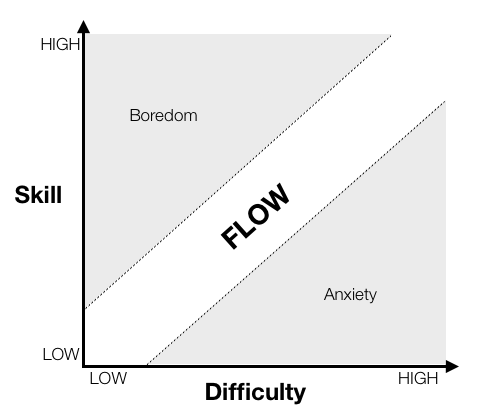
\includegraphics[width=0.60\textwidth]{images/DynamicGameDifficulty.png}
	\caption{Flow, boredom, and anxiety as they relate to task difficulty and user skill level. (2015, January 14). Retreived from: http://www.gamasutra.com/view/feature/166972/, by Csikszentmihalyi, 1990}
	\label{fig:gamedifficulty}
\end{figure}

\subsection{Market}
In the original game design we planned to include a market. A quote from the original design document describes the initial purpose:
\textit{``From the farm you are able to see your inventory. Here you will have an overview of all the items you currently possess. These items can be sold on the market, giving you the revenue they are worth.''}
This feature did not have a high priority at first, as you use the items to start challenges and receive money right away when you harvest. Including the market in the game however provides guidance to the user since it needs certain crops and challenges to be done. 

\subsection{Make body interactive}
\textit{Information is motivation}, from this point of view it would be good to provide more information about the body parts and the use of exercises. One of the future features should therefore provide information about the muscle when it is clicked on in the BODY menu. Next to more information also the challenges and crops that use these muscles have to be shown to make it easy for the user to find the exercises meant for a specific body part. 

\subsection{Statistics Graph}
The BODY menu gives the option to see the statistics to see the completed exercises in the past. To make these statistics more easy to analyse they have to be visually shown with a graph, showing a summary of the gained experience points per body part for a time interval selected by the user. By clicking on a certain point in the graph the finished exercises at that point should be shown.

\subsection{Disclaimer}
The game needs the user to execute all kinds of exercises without prior physical and medical tests. The responsibility of performing the exercises and possible injuries should therefore lay with the user. To warn the users about possible consequences, although they are limited to the minimum, and indicate that the game is on their own responsibility, this should be mentioned in the disclaimer. 

\subsection{Some more fun}
To indicate that the game could really improve the fitness of the user an example would be nice to have. What example is better than the already introduced Phil, an old man in good shape. We planned to look for ``an old photo'' of our example from the time before he was exercising and while he was exercising. With his extensive experience he can tell about his experience and what he had to do to reach and maintain his current shape. 

\subsection{Personal calibration}
People like a personal approach, not feeling just one among many. A personal approach could motivate the user and could also lead to faster results. The intended personalisation consists of a calibration to adjust the settings considering for example the age, height, arm length, weight, current fitness, etc. This information is first of all usable to improve the precision of the measurement of the sensors. Besides that, also the amount of repetitions of exercises, the types of exercises and feedback could be adjusted.

\subsection{Materials}
Giving the users more freedom to decide what they want could increase fun and engagement. Once users earned plenty of money they should be able to invest it to speed up processes and improve faster. This is why we want to introduce materials. Materials can be bought and help speeding up or unlocking certain processes. For example, buying a plowvercraft speeds up the processes on the farm and therefore a crop could be harvested earlier. 